% Proposed plan
% - OTB in a nutshell
% 



%----------------------------------------------------------------------------------------
%	PACKAGES & THEMES
%----------------------------------------------------------------------------------------

\documentclass[8pt,aspectratio=169]{beamer}

\usepackage{etex}
\mode<presentation> {
\usetheme{Vilanova}
}

\usepackage[english]{babel}
\usepackage[utf8]{inputenc}
\usepackage{array}
\usepackage{graphicx}
\usepackage{booktabs}
\usepackage{amsmath,amssymb,amsthm}
\usepackage{xcolor}
\usepackage{tikz}
\usetikzlibrary{arrows}
\usepackage{pifont}
\usepackage{listings,color}
\usepackage{import}

\definecolor{listcomment}{rgb}{0.0,0.5,0.0}
\definecolor{listkeyword}{rgb}{0.0,0.0,0.5}
\definecolor{listnumbers}{gray}{0.65}
\definecolor{listlightgray}{gray}{0.955}
\definecolor{listwhite}{gray}{1.0}

\AtBeginSection[]
{
\addtocounter{framenumber}{-1}
\begin{frame}
\frametitle{Outline}
\tableofcontents[currentsection]
\end{frame}}

%----------------------------------------------------------------------------------------
%	TITLE PAGE
%----------------------------------------------------------------------------------------
\title{Remote Sensing Image Processing}
\subtitle{What's new in Orfeo ToolBox?}
\author{\textbf{Julien Michel (CNES)}, Manuel Grizonnet (CNES), Victor Poughon (CNES), Yannick Tanguy (CNES), Guillaume Pasero (CS), Rémi Cresson (IRSTEA)}
\date{LPS 2019, May 13th-17th 2018, Milano, Italy}

\pgfdeclareimage[width=1.2\textwidth]{background}{../OTB-General/images/fondsClairSansLogo}
\pgfdeclareimage[height=0.2cm]{cc}{../OTB-General/images/CC-licence.png}
\setbeamertemplate{background}{\pgfuseimage{background}}
\pgfdeclareimage[height=0.6cm]{logoIncrust}{../OTB-General/images/logoIncrust}
\pgfdeclareimage[height=0.6cm]{OSGeo_logo}{../OTB-General/images/OSGeo_logo}
\logo{
\begin{tabular}{p{0.22\textwidth}p{0.58\textwidth}p{0.1\textwidth}p{0.1\textwidth}}
\href{http://www.osgeo.org}{\pgfuseimage{OSGeo_logo}}
& \vspace{-0.03\textwidth} \scriptsize{} % date and event here
& \href{http://creativecommons.org/licenses/by-sa/3.0/}{\pgfuseimage{cc}} & \href{http://www.orfeo-toolbox.org}{\pgfuseimage{logoIncrust}}\\
\end{tabular}
}

\begin{document}
\begin{frame}
\titlepage
\end{frame}

\section{In a nutshell}

  \begin{frame}
    \frametitle{OTB in one slide}

      \begin{itemize}
      \item An \textbf{image processing library} for remote sensing
      \item \textbf{Free and open source software} under Apache v2.0 license (since 6.0, formerly CeCILL-v2)
      \item \textbf{Funded and developed by CNES} (French Space Agency) in the frame
        the development of the Pléiades satellite (and beyond)
      \item A project of OSGeo since 2017
      \item Used at CNES, ESA, mission exploitation platforms,
        remote sensing labs, for teaching\ldots
      \item Written in \textbf{C++} on top of \href{www.itk.org}{ITK} (medical image
        processing)
      \item Built on the shoulders of giants (GDAL, OSSIM, OpenCV\ldots)
      \item \textbf{Big Data} capable, thanks to built-in streaming and multithreading
      \end{itemize}

    
    \begin{center}
      {\huge\textcolor{red}{\href{http://www.orfeo-toolbox.org}{orfeo-toolbox.org}}}
    \end{center}
  \end{frame}

    \begin{frame}[fragile]
      \frametitle{Getting started}
      
      \begin{center}
        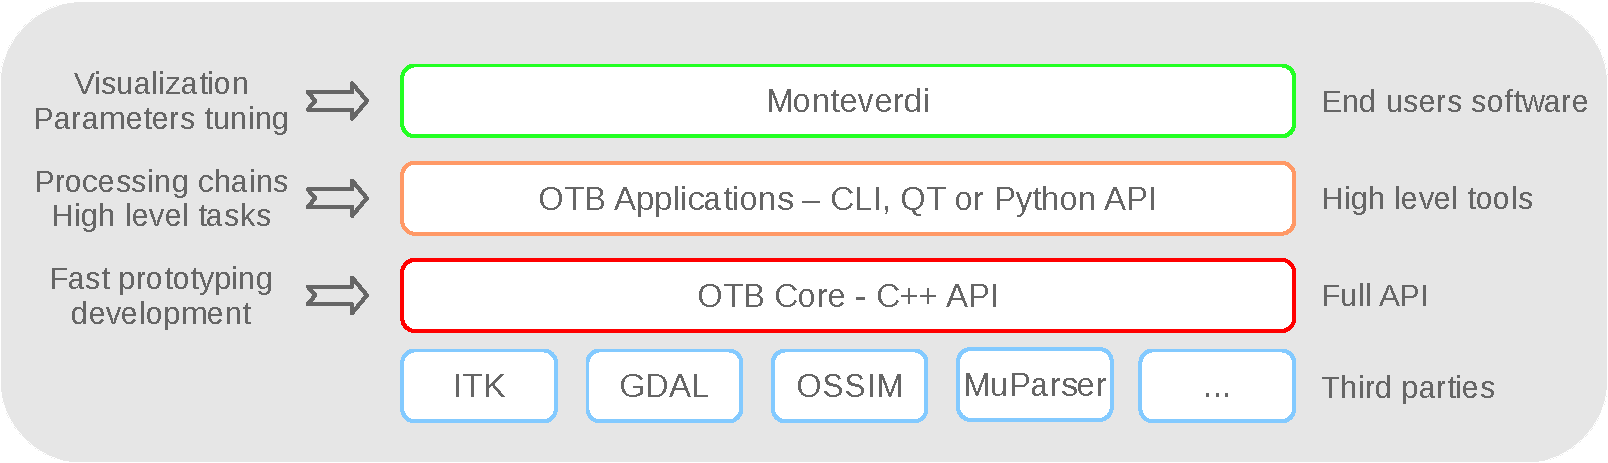
\includegraphics[width=0.8\textwidth]{../OTB-General/images/sandwich.pdf}

        \vspace{0.2cm}
        
        \hspace*{-15mm} \includegraphics[height=2.5cm]{../OTB-General/images/mayotte_mad.png}
        \includegraphics[height=2.5cm]{../OTB-General/images/saint_paul_lsd.png}
        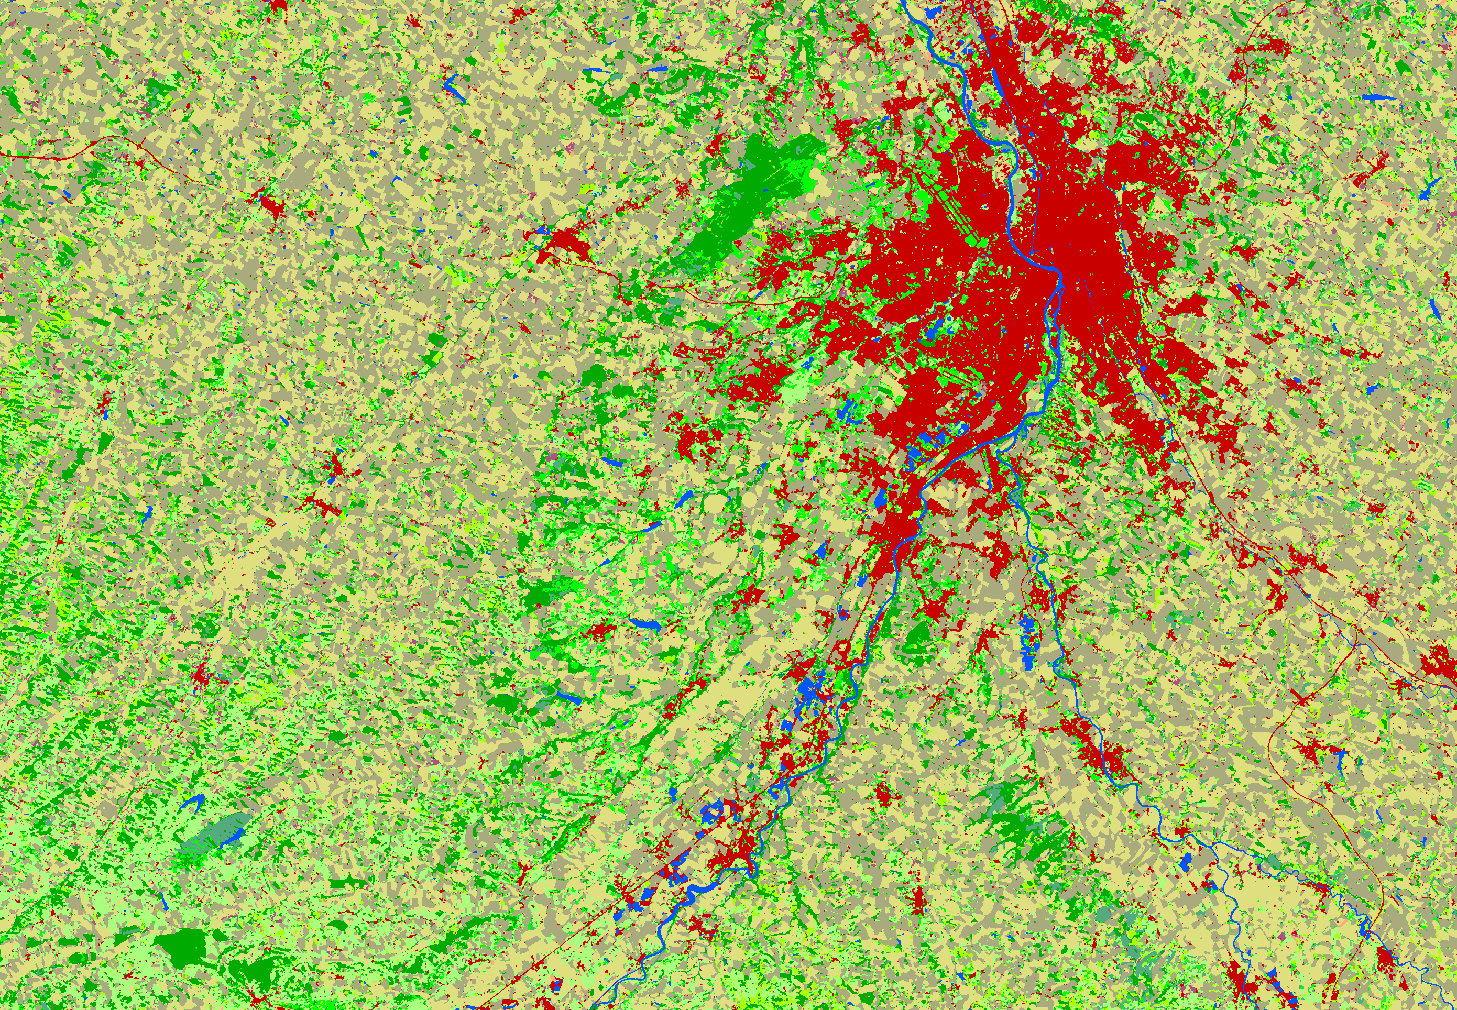
\includegraphics[height=2.5cm]{../../Courses/org/WorkshopGuide/Images/final_classification.png}
        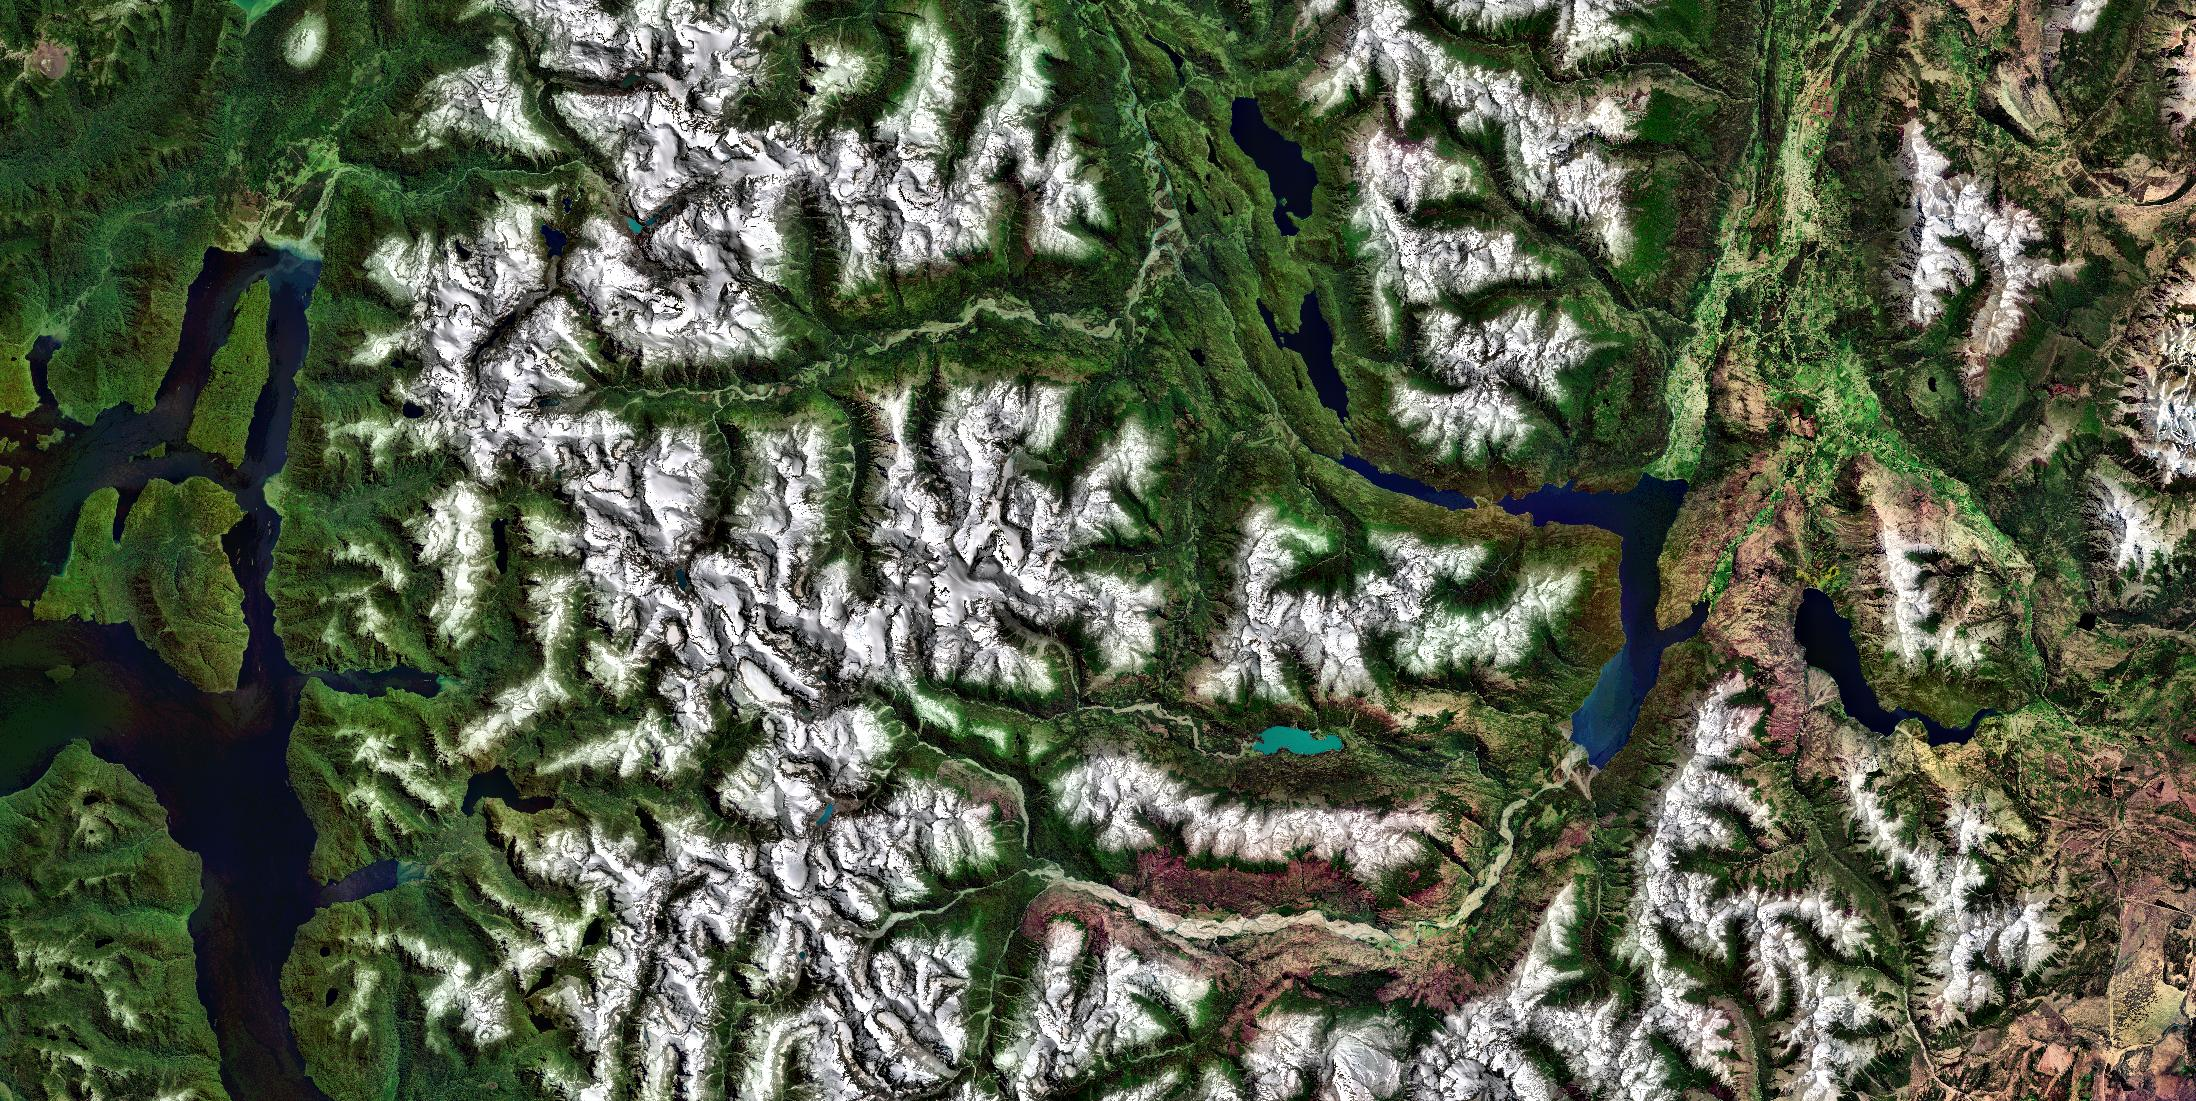
\includegraphics[height=2.5cm]{../OTB-General/images/image4_glob_each_lim20_8b_sub.jpg}

        


      \end{center}
    \end{frame}

      \begin{frame}
        \frametitle{Getting helped}
        \begin{center}
        \begin{small}
          \vspace{0.2cm}
        \hspace*{-13mm}\begin{tabular}{cc}
        Cookbook: \url{https://www.orfeo-toolbox.org/CookBook/} & Forum: \url{https://forum.orfeo-toolbox.org}\\
          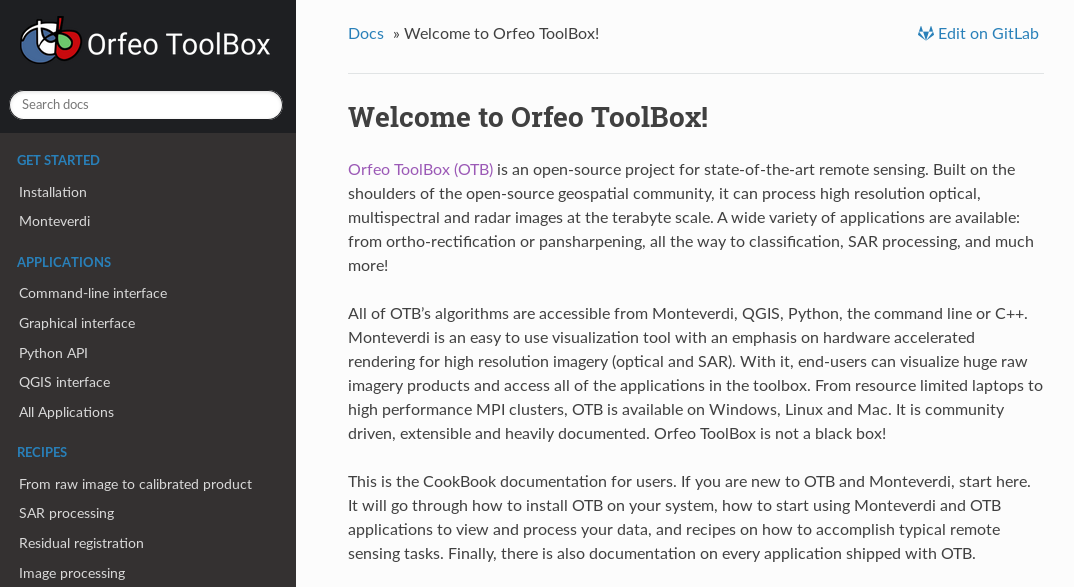
\includegraphics[height=4cm]{cookbook.png} & 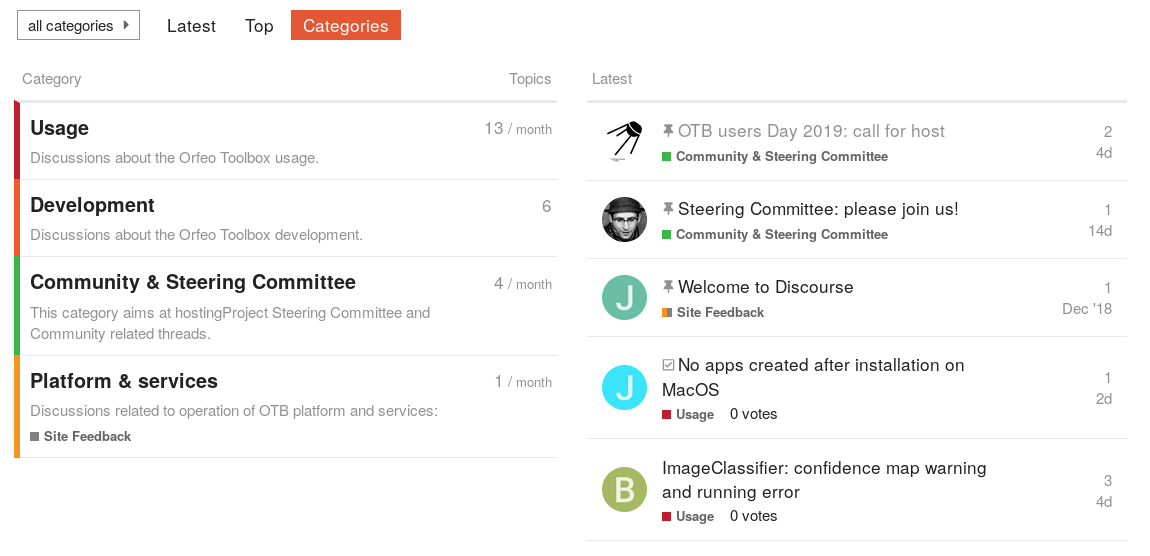
\includegraphics[height=4cm]{discourse.png}\\
      \end{tabular}
        \end{small}
      \end{center}
    \end{frame}

    \begin{frame}
    \frametitle{Remote modules}

    \begin{columns}
      \column{0.66\textwidth}
    \begin{block}{What they are}
      \begin{itemize}
      \item Features developed and maintained by users
      \item Integrate perfectly within OTB: tested, and sometimes shipped in binary packages!  
      \end{itemize}
    \end{block}
    
    \begin{block}{Flagship remote modules}
      \begin{itemize}
      \item OTBTF: Brige Tensor Flow and OTB classification framework! (Rémi Cresson, IRSTEA)
      \item Mosaic: Build mosaic from multiple images (Rémi Cresson, IRSTEA)
      \item DiapOTB: Sentinel1 interferometry with OTB! (CNES)
      \item GRM: Generic Region Merging segmentation algorithm! (Pierre Lassalle PHD)
      \item LSOBIA: GRM segmentation algorithm on clusters! (CNES)
        
      \end{itemize}
      
    \end{block}
    \column{0.33\textwidth}
    \begin{center}
    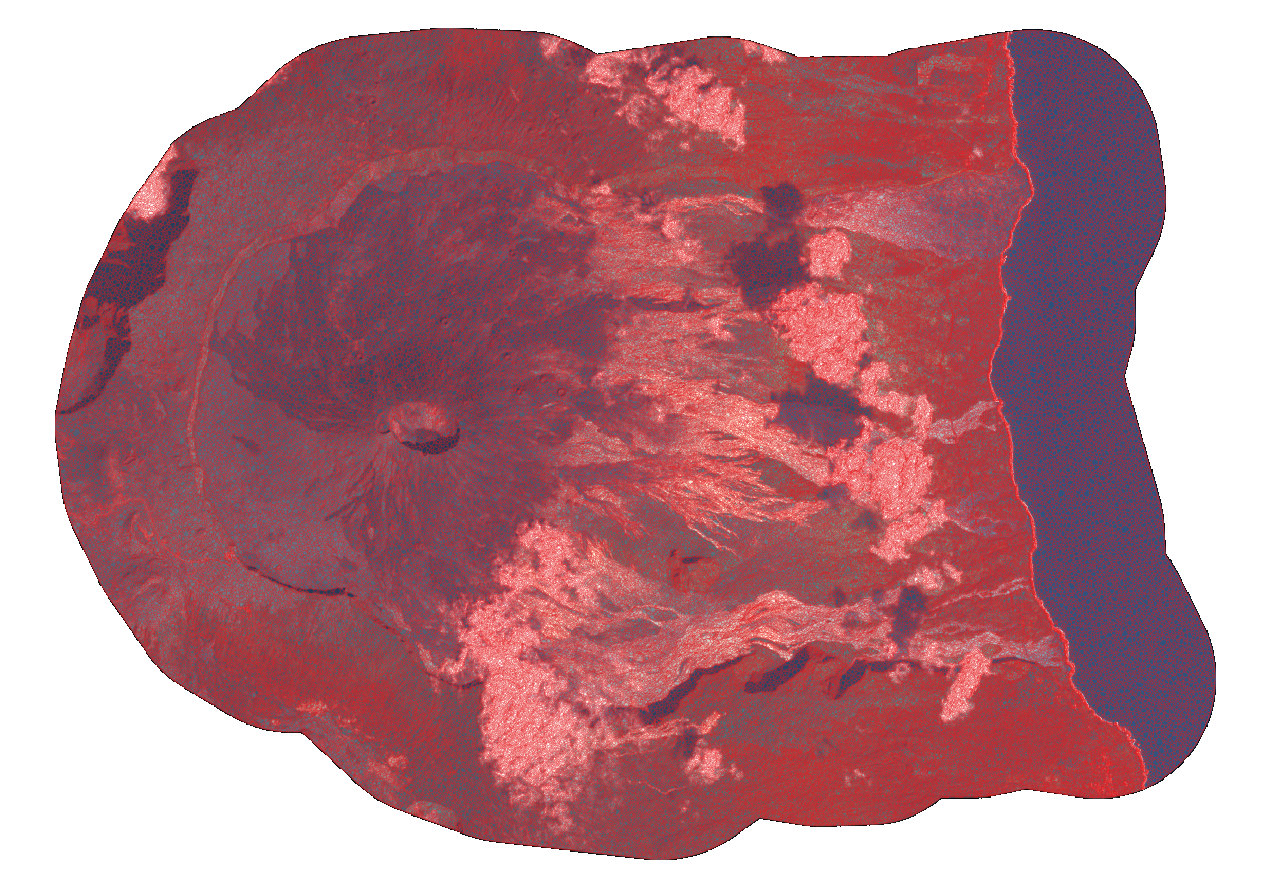
\includegraphics[width=0.9\textwidth]{seg_reunion.png}\\
    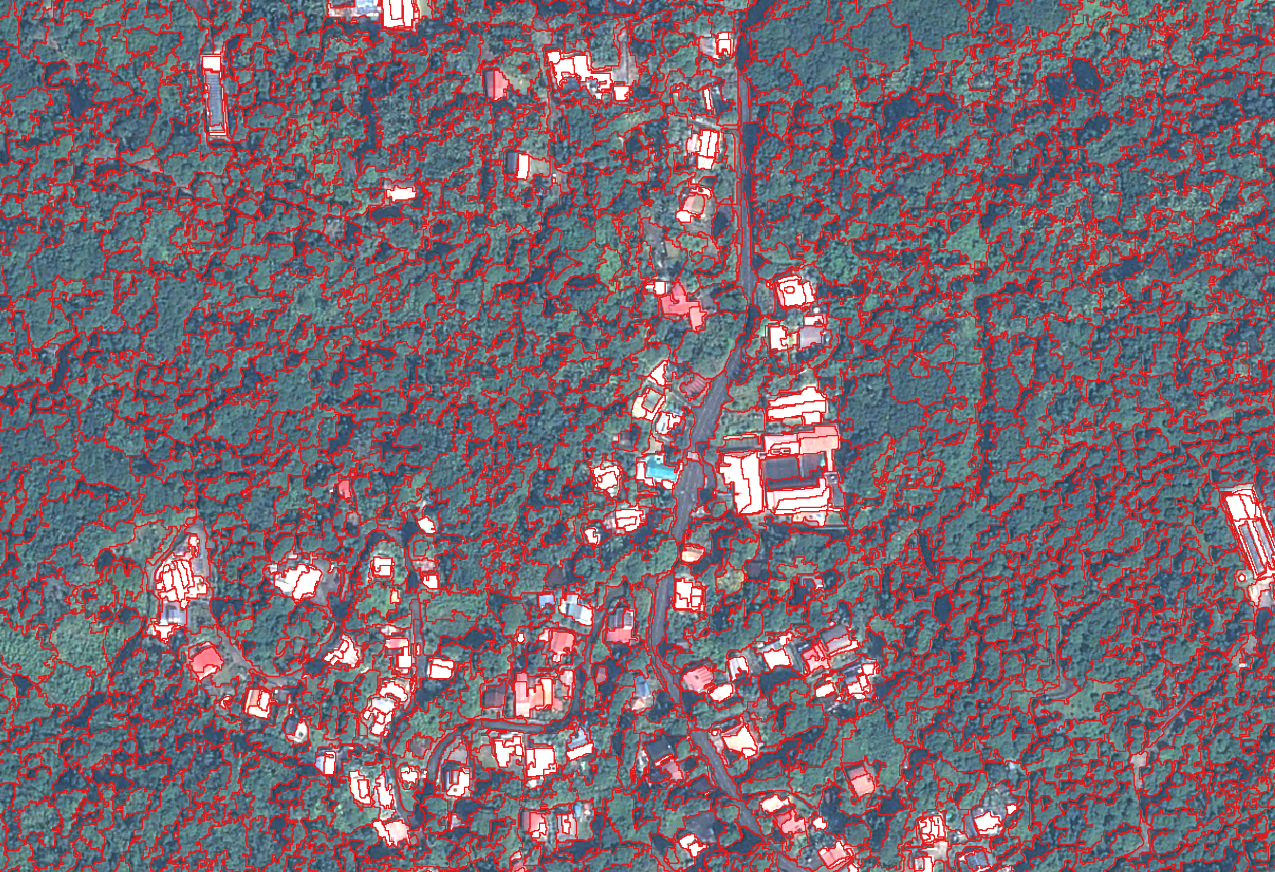
\includegraphics[width=0.7\textwidth]{seg_reunion_zoom.png}\\
    \begin{small} 3 221 860 polygons segmented in 14m on 32 cluster nodes with LSOBIA \end{small}
    \end{center}
    \end{columns}

    
    
    \end{frame}

\section{OTB and Sentinel data}

\begin{frame}
  \frametitle{OTB and Sentinel 1}
  \begin{columns}
    \column{0.6\textwidth}
    \begin{block}{Sentinel 1 support}
      \begin{itemize}
      \item Sensor modeling / ortho-rectification
      \item Gamme Beta-nought radiometric calibration
      \item Deburst of IW products
      \end{itemize}
    \end{block}

    \begin{block}{S1 Tiling tool}
      \begin{itemize}
      \item Radiometric calibration
      \item Orthorectification of S1 images on S2 MGRS grid
      \item Multi-temporal speckle reduction
      \item Operated on PEPS on demand processing service
      \item \small{\url{http://www.cesbio.ups-tlse.fr/multitemp/?p=14905}}
      \item \small{\url{http://tully.ups-tlse.fr/koleckt/s1tiling/tree/master}}
      \end{itemize}
      \end{block}

    \column{0.4\textwidth}
    \begin{center}

      \small{See poster on friday, 12:20-2:00, South hall, floor 0\\ \emph{Analysis Ready Data session}}\\
      \vspace{0.5cm}
      %\includegraphics[width=0.4\textwidth]{S1-time-series1.png}\\
      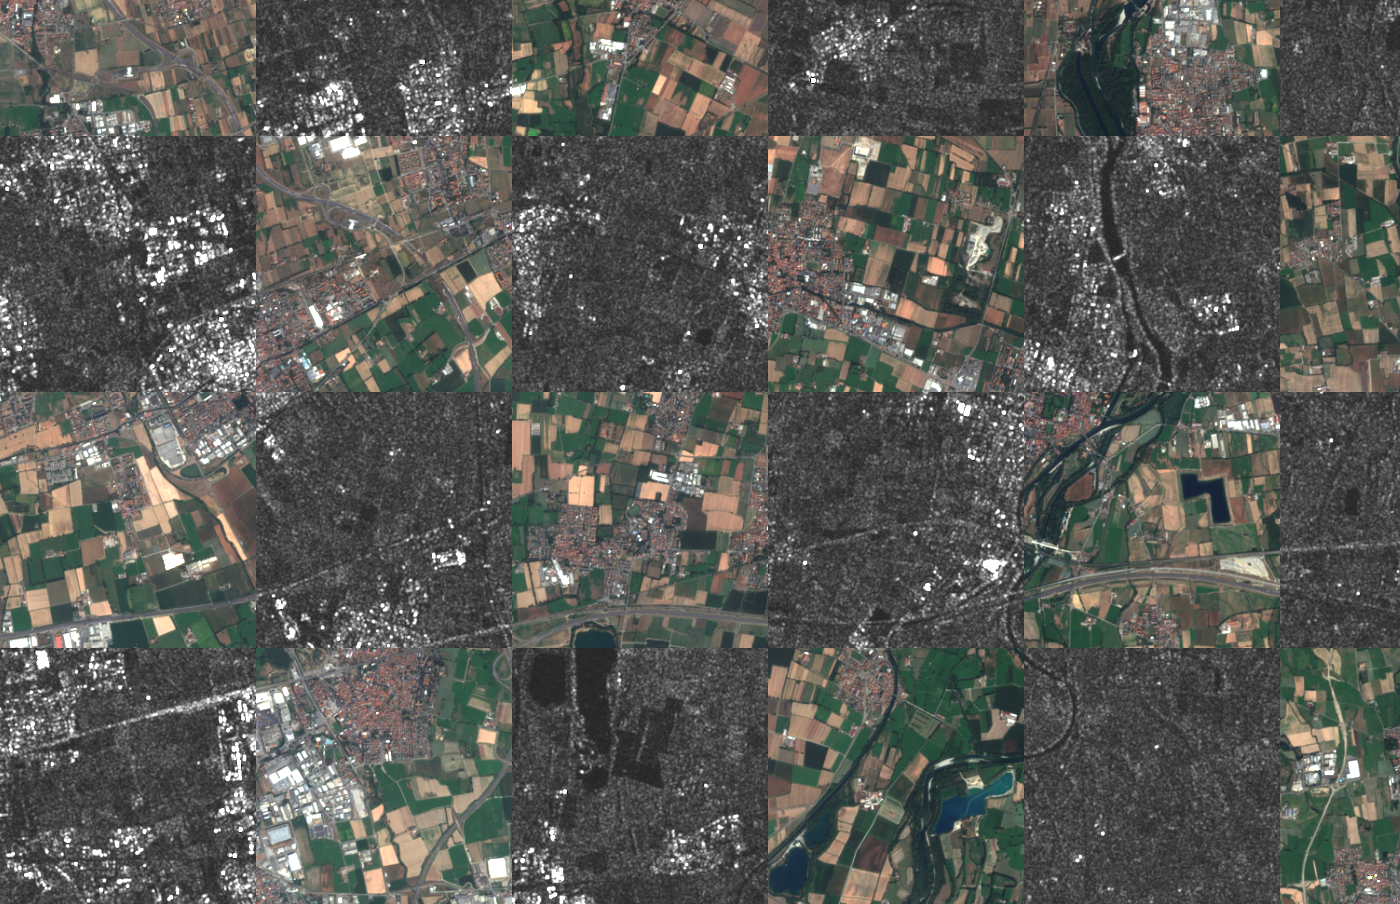
\includegraphics[width=\textwidth]{s1_s2.png}
    \end{center}
  \end{columns}
    
    
    \end{frame}

    \begin{frame}
    \frametitle{OTB and Sentinel 1 cont.}

    \begin{block}{DiapOTB remote module}
      \begin{itemize}
      \item SAR interferometry with OTB
      \item Port of Diapason legacy code
      \item Support of SM and IW SLC products
      \item \small{\url{https://gitlab.orfeo-toolbox.org/remote_modules/diapotb}}
      \end{itemize}
    \end{block}
    
    \end{frame}

      \begin{frame}
        \frametitle{OTB and Sentinel 2}

        \begin{block}{Did you know ?}
          \begin{itemize}
          \item Every Sentinel2 image went through OTB in the Image Processing Facility
          \item Maja L2A processor operated by Theia is written in OTB
          \item Most of OTB applications and algorithms will work out of the box with Sentinel2 imagery
          \end{itemize}
        \end{block}
        \begin{block}{Useful applications for Sentinel2}
          \begin{itemize}
          \item \textbf{RadiometricIndices:} To compute 21 different radiometric indices at once
          \item \textbf{ContrastEnhancement:} To get a nice rendering for publishing
          \item \textbf{Superimpose:} To upsample lower resolution bands 
          \item \textbf{MultivariateAlterationDetector:} To detect changes between two dates
          \item \textbf{ZonalStatistics:} Get statistics for your Sentinel2 image for each shape in your vector file
            \end{itemize}
          \end{block}
      \end{frame}
      
      \begin{frame}
        \frametitle{OTB and Sentinel 2 cont.}
        \begin{columns}
          \column{0.55\textwidth}

          \begin{center}
          \textcolor{red}{Some key components of \textbf{Iota2} Land Cover Mapping chain}\\
          \small{See talk on thursday, 11:40 - 11:55, Space 2, floor 0\\ \emph{Land Cover Regional to Global session}}
          \end{center}

          \begin{block}{Sampling for supervised classification}
            \begin{itemize}
            \item Fair selection of samples within polygons
            \item Strategy: class balance, fixed number of samples \ldots
            \item Takes into account no data and masks
            \item Output a point vector file with pixel values as attributes
            \end{itemize}
        \end{block}
        
        \begin{block}{Temporal Gap-Filling remote module}
          \begin{itemize}
          \item \small{\url{http://tully.ups-tlse.fr/jordi/temporalgapfilling}}
          \item Interpolate invalid pixels with various strategy
          \item Temporal resampling on a set of dates
          \end{itemize}
          
        \end{block}
        
        \column{0.45\textwidth}
        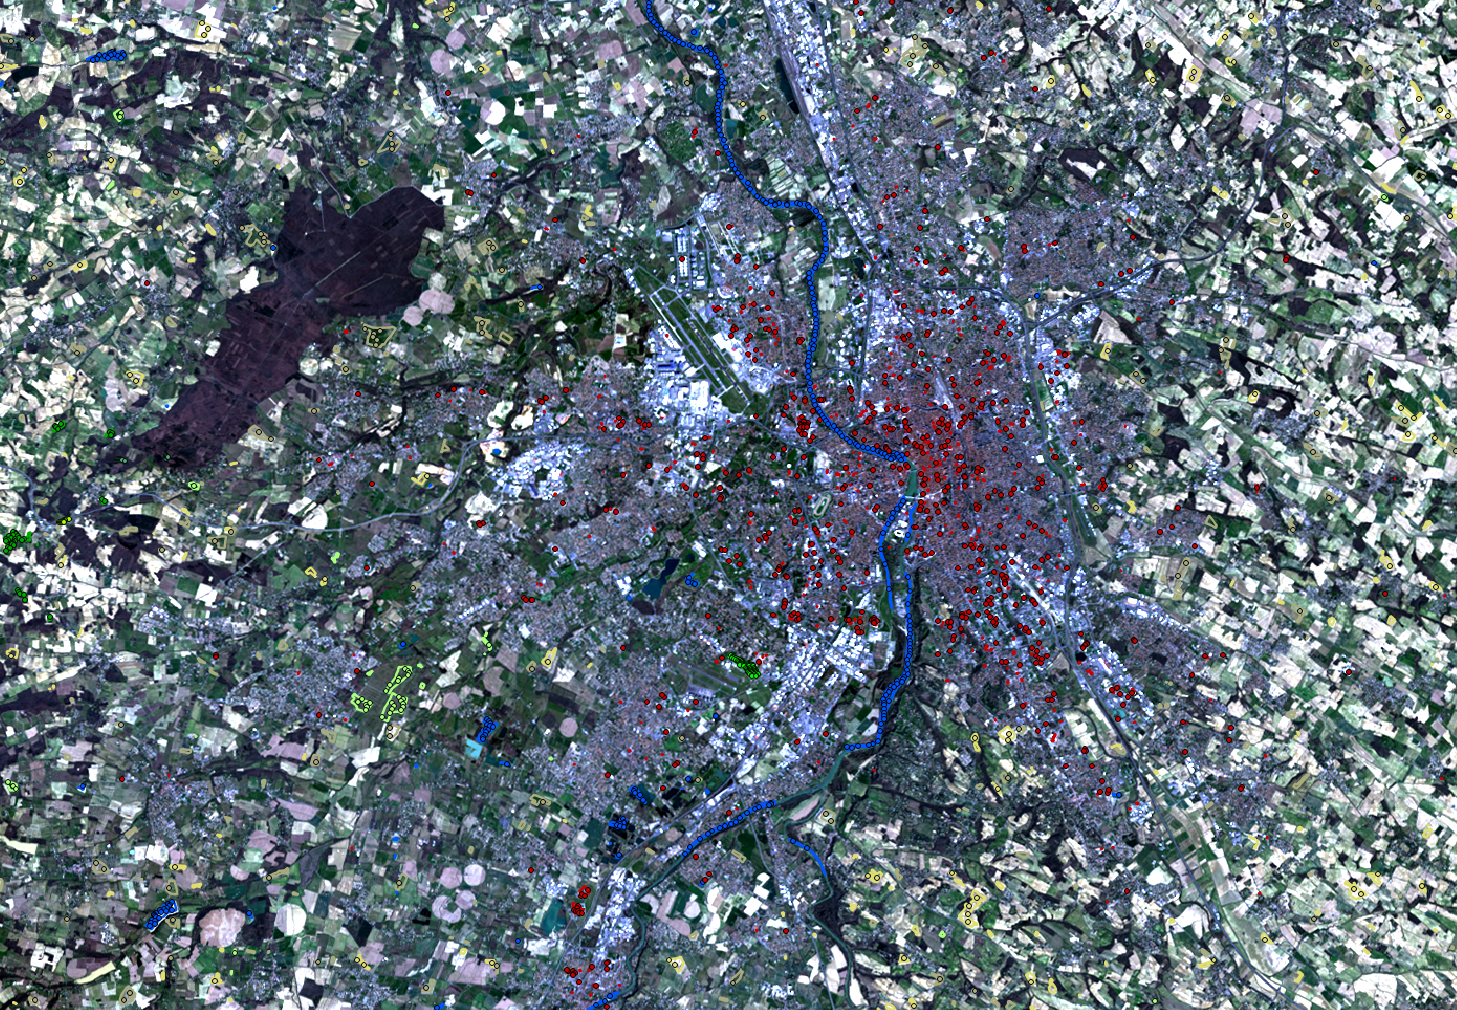
\includegraphics[trim={0 5cm 0 5cm},width=\textwidth]{../../Courses/org/WorkshopGuide/Images/samples_selection.png}\\
          \includegraphics[width=\textwidth]{../Atelier-MOSO-2016/images/samples-extraction.png}
        \end{columns}        
    \end{frame}
  
\section{New in OTB 7.0}

    \begin{frame}[fragile]
    \frametitle{7.0 changes highlight}
    \begin{center}
      Latest release: 6.6.1 on 2018.12.12 (\small{\url{https://www.orfeo-toolbox.org/download/}})\\
      \vspace{0.1cm}
      \color{red}{7.0.0 release schedule: 2019.06}
    \end{center}
    \begin{itemize}
    \item Long term work on cleaning and optimizing the code:
      \begin{small}
      \begin{verbatim}
  $ git diff --shortstat release-6.6 Modules/ Examples/ Documentation/ SuperBuild/
    5586 files changed, 161115 insertions(+), 500972 deletions(-)
      \end{verbatim}
      \end{small}
    \item No more software guide: everything is now in the \textbf{CookBook}, which has been enhanced,
    \item Nice new features such as \textbf{ZonalStatistics} application, revamped \textbf{RadiometricIndices} application \ldots
    \item A Full hyperspectral story with new applications (\textbf{LocalRxDetector}, \textbf{EndmemberNumberEstimation}) and a Cookbook recipe for hypespectral imaging
    \item Lots of improvement in applications graphical user interfaces
    \item Better integration wihtin \textbf{QGis}
    \item Tons of bugfixes!
      
    \end{itemize}

    \end{frame}

    \begin{frame}[fragile]
    \frametitle{The OTB code factory / Contributing}

    \begin{columns}
      \column{0.5\textwidth}
      \begin{block}{Report bugs}
        \begin{itemize}
        \item First (and most important) kind of contribution
        \item Open issues on gitlab
        \item Use the template, and be precise!
        \item Don't be afraid of reporting false bugs!
        \end{itemize}
      \end{block}

      \begin{block}{Help others}
        \begin{itemize}
        \item We need help to answer questions on forum!
        \item \small{\url{https://forum.orfeo-toolbox.org/}}
        \end{itemize}
      \end{block}
    
      \column{0.5\textwidth}
      \begin{block}{Submit Merge Requests}
        \begin{itemize}
        \item Merge requests on gitlab (also accepted on Github)
        \item Full contribution process in CONTRIBUTING.md
        \item A new CI service is being set-up
        \item You can edit documentation in-place (RST)!
        \end{itemize}
      \end{block}

      \begin{block}{Become a PSC member}
        \begin{itemize}
          \item Become an OTB evangelist
          \item Vote a few important decisions each year
          \item Organize and teach training sessions \ldots
        \end{itemize}
      \end{block}
      
    \end{columns}

    \begin{center}
      \large{\textbf{Thank you for your attention! Questions?}}
      
    \end{center}
    
    \end{frame}


\end{document}
